\documentclass[a4paper]{article}

%% Language and font encodings
\usepackage[T2A]{fontenc}
\usepackage[english, russian]{babel}
\usepackage[utf8x]{inputenc}
\usepackage{listings,xcolor}

%% Sets page size and margins
\usepackage[a4paper,top=1cm,bottom=2cm,left=1.5cm,right=1.5cm,marginparwidth=1.75cm]{geometry}

%% Useful packages
\usepackage{amsmath}
\usepackage{amssymb}
\usepackage{graphicx}
\usepackage[colorinlistoftodos]{todonotes}
\usepackage[colorlinks=true, allcolors=blue]{hyperref}
\usepackage{array}

\newcolumntype{C}[1]{>{\centering\arraybackslash}m{#1}}

\title{Курсовая работа по <<Продвинутым алгоритмам>>}
\author{Алексей Латышев, группа M4139}

\DeclareMathOperator*{\argmax}{arg\,max}
\DeclareMathOperator*{\argmin}{arg\,min}
\begin{document}
\maketitle

В рамках курсовой работы нужно было реализовать структуру данных <<Dynamic
connectivity online>>, которая хранит в себе граф и умеет обрабатывать следующие запросы:
\begin{itemize}
\item $link(u, v)$ --- провести еще не проведенное ребро $(u, v)$
\item $cut(u, v)$ --- удалить проведенное ребро $(u, v)$
\item $are\_connected(u, v)$ --- проверить, лежат ли вершины $u$ и $v$ в одной
  компоненте связности    
\end{itemize}

Для этого в качестве структуры с операциями $(merge, split, get\_id)$ на
связных списках было реализовано декартово дерево.

Затем с использованием этой структуры было реализовано дерево эйлерова обхода.
Это структура данных, отвечающая на те же запросы, что и dynamic connectivity,
однако требующая инварианта, что хранимый граф --- лес.

После этого была реализована требуемая структура данных. Код проекта можно найти
на \href{https://github.com/alex-700/dynamic-connectivity}{github}. Весь код
написан в единственном хедере в директории \emph{include}. Тесты и попытки
провести $benchmark$ можно найти в директориях \emph{tests} и \emph{benchmarks}
соответственно.

Результаты бенчмарка можно увидеть на графиках на следующей странице.
\begin{figure}[h]
  \centering
  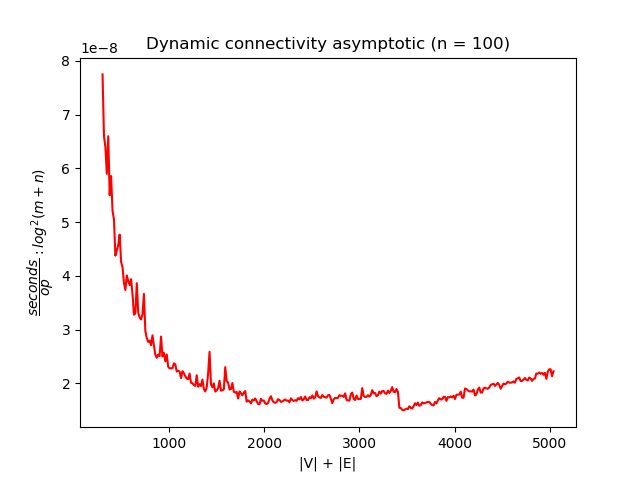
\includegraphics[width=0.5\textwidth]{graphics100.png}
  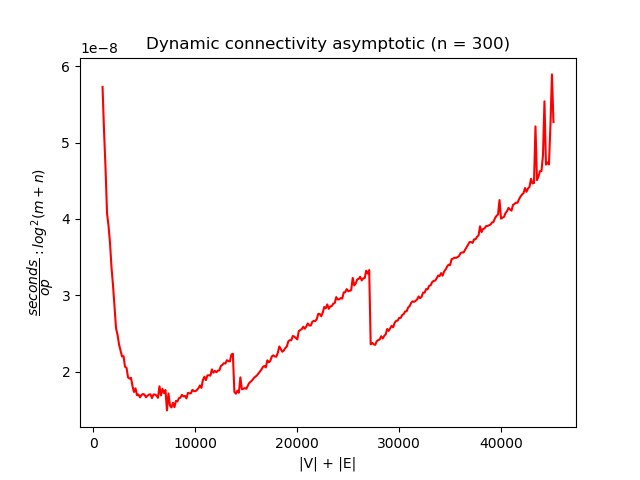
\includegraphics[width=0.5\textwidth]{graphics300.png}
  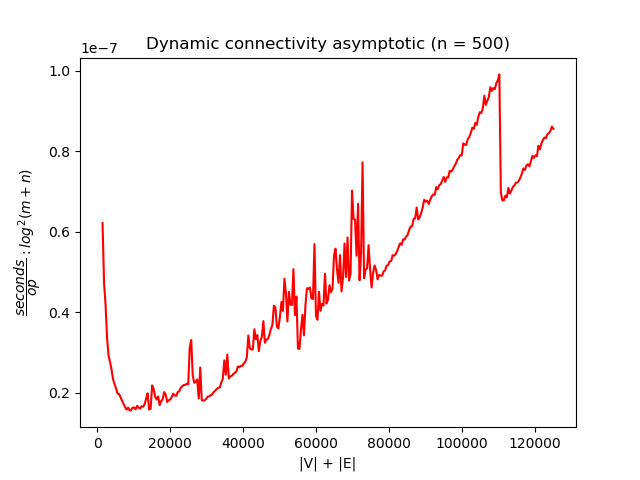
\includegraphics[width=0.5\textwidth]{graphics500.png}
\end{figure}

Эти графики показывают отношение среднего времени работы одной операции к
предполагаемой асимптотике $O(log^2(|V| + |E|))$. В качестве исследуемого теста
использовался сценарий, когда мы последовательно добавляем $|E|$ рандомных
ребер, а потом всех их удаляем. В принципе, видно, что график почти константа.
Скачок в начале объясняется тем, что когда ребер сравнимо с количеством вершин,
то все запросы превращаются к запросам в дерево эйлерова обхода, в то время как
при большем количестве ребер большинство запросов обрабатывается
намного быстрее. А скачок при больших $m$ происходит из-за рандомизированной
оценки на время запросов к декартову дереву. 

\end{document}

%%% Local Variables:
%%% coding: utf-8
%%% mode: latex
%%% TeX-master: t
%%% TeX-command-extra-options: "-shell-escape"
%%% TeX-engine: 
%%% End:spacemacs

